
\documentclass{article}

\usepackage[activate={true,nocompatibility},final,tracking=true,kerning=true,spacing=true,factor=1100,stretch=10,shrink=10]{microtype}
% activate={true,nocompatibility} - activate protrusion and expansion
% final - enable microtype; use "draft" to disable
% tracking=true, kerning=true, spacing=true - activate these techniques
% factor=1100 - add 10% to the protrusion amount (default is 1000)
% stretch=10, shrink=10 - reduce stretchability/shrinkability (default is 20/20)

\usepackage[utf8]{inputenc}
\usepackage{amssymb}
\usepackage{amsmath}
\usepackage{mathtools}
\usepackage{svg}
\usepackage{graphicx}
\usepackage[superscript, biblabel, nomove]{cite}
\usepackage[hidelinks]{hyperref}
\usepackage{cleveref}
\usepackage{tikz}
\usepackage{pgfplots}
\usepackage{datetime}
\usepackage{color}

\pgfplotsset{width=7cm,compat=1.9}

% use "\head" to define table heading formatting
\newcommand{\head}[1]{\textnormal{\textbf{#1}}}

% Use § for sections
\crefformat{section}{\S#2#1#3}
\crefformat{subsection}{\S#2#1#3}
\crefformat{subsubsection}{\S#2#1#3}

\usepackage{appendix}

% == Remove or comment these out for release
%\usepackage{todonotes}
%\usepackage{draftwatermark}
%\SetWatermarkText{DRAFT}
%\SetWatermarkScale{3}
% ==

\usepackage[utf8]{inputenc}
\usepackage[english]{babel}
\usepackage{amsthm}

% Make itemize bullets slightly smaller
\renewcommand\labelitemi{{\boldmath$\cdot$}}

\newtheorem{theorem}{Theorem}
\theoremstyle{definition}
\newtheorem{definition}{Definition}[section]

\newtheorem{thm}{The`orem}[section] % the main one
\newtheorem{lemma}[thm]{Lemma}

\theoremstyle{plain} % just in case the style had changed
\newcommand{\thistheoremname}{}
\newtheorem{genericthm}[thm]{\thistheoremname}
\newenvironment{namedthm}[1]
  {\renewcommand{\thistheoremname}{#1}%
   \begin{genericthm}}
  {\end{genericthm}}


\begin{document}

% Macros
% nil

\title{Enosi Green Paper\\ v0.2}
\author{Samuel Brooks, Matthew Hale, Steve Hoy}
\date{}

\maketitle

\hfill

\begin{abstract}
\noindent Modern energy markets are structurally inefficient, resulting in higher-than-neccessary electricity prices and frustration of investment into appropriate renewable infrastructure.
Grid 2.0 technologies, coupled with cheap, renewable solar, can optimise the generation and distribution architecture of aging energy networks and slash cost from the energy stack.
Critically, electricity companies in commercial competition with one another within a given energy market naturally segment the customer base, resulting in structurally sub-optimal risk management for the purchase and provision of electricity. By using distributed ledger technology, Enosi proposes to split this business model into two, thereby creating a competitive market for load profiles and optimised credit risk, resulting in lower electricity prices for end consumers.
\end{abstract}
\vspace{20mm}
\begin{center}
  %\color{gray}
  \small{\textit{\today}}
\end{center}

% \todo[inline]{Incorporate white paper criticisms.}

\pagebreak

\tableofcontents

% == Remove or comment out this section for release
% \pagebreak
% \section{TODO}
% \listoftodos{}
% ==

\pagebreak

%\input{tex/introduction}
%\input{tex/design_considerations}
%\input{tex/system_description}



% \appendix
% \appendixpage
% \addappheadtotoc
%\input{tex/alternative_approaches}
%\input{tex/system_variables}

%\bibliography{tex/citations}
%\bibliographystyle{plain}


\section{Introduction}

Globally, it is now clear that a number of issues have resulted from a centralised power generation architecture, including the stimulation of the use of fossil fuels in order to extend the life of existing assets, a power-inefficient transmission system, and regulation which supports incumbency and stymies innovation. Even though Australia is one of the most deregulated energy markets in the world, it structurally inhibits local (distributed) generation and consumption. \\

\noindent Enosi seeks to provide the means for small and startup energy businesses and not-for-profit entities to compete in established markets. Providing such an equal opportunity fosters competition with incumbent players, allowing more competitive and more relevant services to be offered to energy consumers, such as the facility for localised peer-to-peer energy trading, control over the provenance of their electricity, and transparency of cost. \\

\noindent The key enabler for this shift is the ability for all actors in a retail energy market to access a shared understanding of (i) energy usage data and (ii) pricing and settlement logic that acts over that data. Distributed ledger technology enables us to build such shared data and logic systems, including standardised software and business process workflows. Indeed, cryptographically-secure methods of sharing both information and logic are the only way to orchestrate the necessary cooperation to achieve the economies of scale necessary to provide localised services and price-efficient community energy. By taking full advantage of distributed ledger technology, as well as “Grid 2.0” technologies such as smart meters, we can create very efficient networks of interconnected retailers, Neo-retailers and customers to both cooperate and compete with one another.\\

\noindent Enosi is developing a distributed ledger software platform to provide the tools and network effect to enable small and community-based actors to disrupt established energy market players. It is a not-for-profit foundation developing this platform as a Software-as-a-Token model, and will be initially funded as an ICO. While the software will be made open source, the token is required to access individual energy networks (geographical markets).\\

\noindent "We are here to change the electricity industry, because the incumbents won’t."\\
- Stefan Jarnson, Enosi Project




\pagebreak
\section{Solution Design}

\subsection{Problem Space}

Currently, there exists two key structural inefficiencies in modern energy markets: fragmented risk management, and misaligned investment incentives. We explore these in turn.

\subsubsection{Inefficient buying risk management}

The first is the segregation of loads due to customer segmentation within a market; most customers within an energy market are contracted to a small number of large energy companies to provide their electricity. These companies manage their own buying risk with the wholesale electricity market (power generation companies sell into this wholesale market). Modern electricity regulation in most jurisdictions globally require continuity of service for end-consumers, and this means that protections exist for generators against the interposing energy retailer mismanaging its balance sheet and being unable to pay generators for the electricity it is required to buy and supply to its customers. This protection takes the form of a credit or bond held on trust with the local regulator in the event that the retailer cannot pay its bill to the wholesale market. However even within this context, energy retailers still seek to make a profit, and this comes from improving the efficiency of their risk management in buying power from the wholesale market and selling it to end consumers. \\

\noindent Because the market is segregated between these energy retailers who are in competition, an optimal risk management strategy is never able to be achieved; the most efficient scenario is one where all customer load profiles, both commercial and residential, are aggregated to produce a ‘flat’ a demand as possible, making the prediction of what electricity is necessary to purchase as accurate as possible. A completely predictable load profile is one which can be easily satisfied, and the greater the number of customers within a market smooths out this load profile making it more predictable.

\subsubsection{Grid management incentives}

In addition, incumbent companies in some jurisdictions are not appropriately incentivised to maintain an inefficient grid. Reduction of capital expenditure for the utility.

Nelson bay example.

<steve to add info on this>.

\subsection{Solution Space}

The key to unlocking value in these energy markets is to reconfigure the market with a fundamentally more efficient set of actors. Specifically, we propose decomposing the traditional energy retailer into two distinct parts: a wholesale Licensed Supplier, and a Neo-retailer.\\

\noindent \textbf{Licensed Supplier} - a company or other entity who buys electricity from the wholesale market and sells it into the retail market, typically via a Neo-retailer. Licensed Suppliers are required to abide by existing prudential regulations, including holding capital to protect creditors (electricity generation businesses) against a failure of their credit risk operations.\\

\noindent \textbf{Neo-retailer} - a company or other entity which specialises in providing customer-facing services, including customer acquisition, metering, billing, and ancillary services such as peer-to-peer energy functions. Neo-retailers may be operated by anyone, including not-for profit community groups, or tangentially related business (such as electric vehicle manufacturers) who can market more specific value propositions to their customers.\\

\vspace{2mm}

\begin{center}
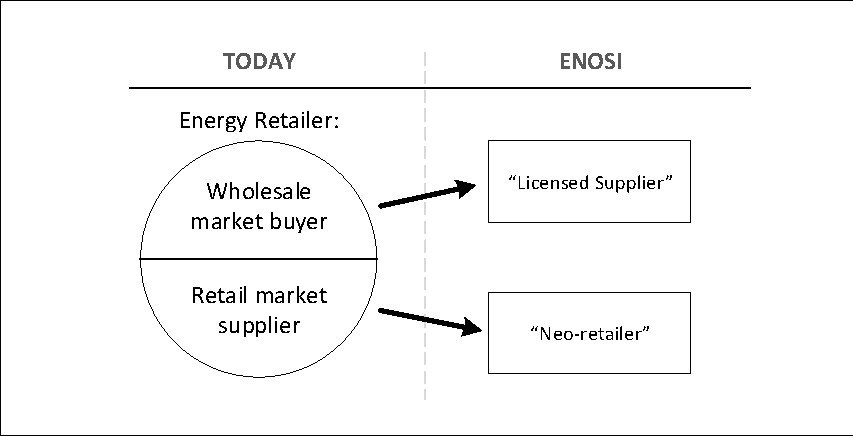
\includegraphics[width=250pt]{/home/samuel/dev/block8/green-paper/enosi-retailer-split.pdf}\\
\end{center}


\noindent The effect of this will be to:

\begin{itemize}
\item{Create a single marketplace for Neo-retailers to acquire customers, and for Neo-retailers in turn to publically advertise and on-sell their unique customer load profile. This enables Licensed Suppliers to compliment their sell profile in order to optimise their buying profile, and in turn offer more competitive pricing to the Neo-retailer.}
\item{Reduce the cost of customer management functions by supporting not-for-profit entities to act as Neo-retailers. Such entities will be structurally more competitive than traditional for-profit service companies, resulting in cheaper electricity prices for end customers.}
\item{Create a more diverse set of Neo-retailers more able to satisfy customer subgroups.}
\item{Accelerate the use of smart metering as Neo-retailers can form around this technology to offer even cheaper and more efficient retailing services by removing the need for manual meter-reading.}
\item{Accelerate the use of distributed generation (e.g. rooftop solar) as it becomes easier for actors to enter the market and offer peer-to-peer services.}
\end{itemize} 

\noindent Creating such a network is achievable by using distributed ledgers to efficiently share metering and customer data as well as adhere to a common standard for the energy retailing stack. Having all market actors running common software for standardising basic energy information (e.g. metering) and logic (e.g. billing) means that interoperation between market players becomes possible (integrating every disparate system together, or creating a separate for-profit company dedicated to interfacing between every system would be impractical). It is only via the creation of a not-for-profit foundation, run by individuals who are incentivised to improve the value of the network, does such a singular network become possible. \\

\vspace{2mm}
\begin{center}
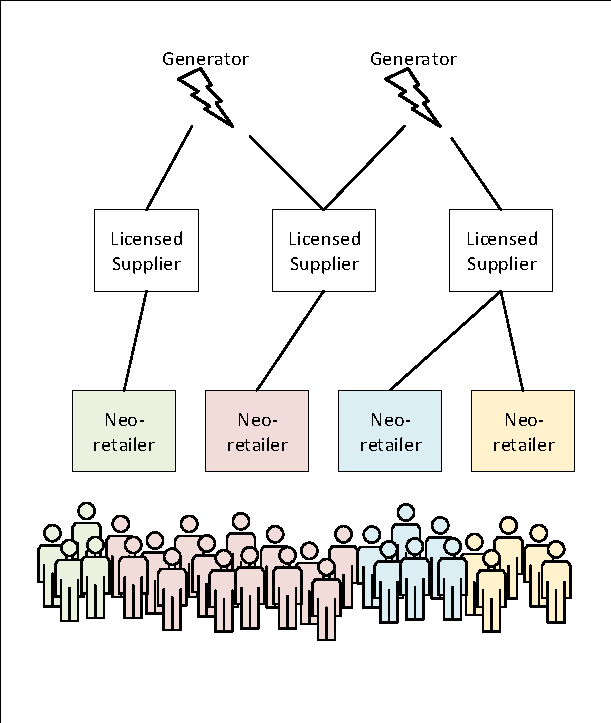
\includegraphics[width=250pt]{/home/samuel/dev/block8/green-paper/enosi-stack.pdf}
\end{center}
\vspace{3mm}

\noindent As the network grows and matures over time, this will create further incentives for Licensed Suppliers to cooperate and ultimately aggregate into super-operators in order to continue to take advantage of sell-side aggregation of load profiles. Setting up such a network will naturally break down the fragmented market through these continued cooperative agreements. Because Neo-retailers are in custody of their own data and logic (including a customer identity) and that within the market Neo-retailers are able to easily switch between their electricity supplier, this aggregation will not be anti-competitive. \\

\vspace{2mm}
\begin{center}
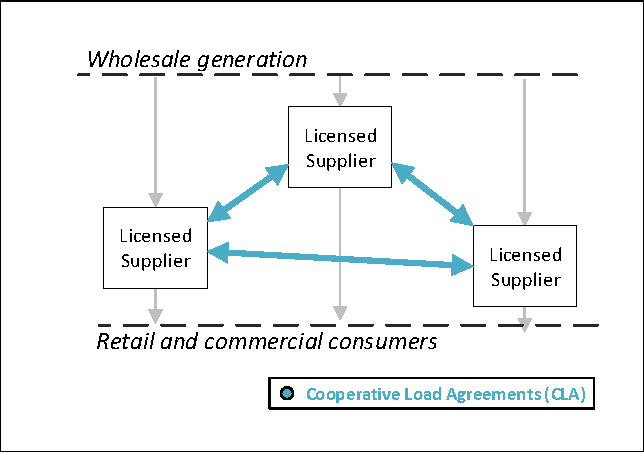
\includegraphics[width=300pt]{/home/samuel/dev/block8/green-paper/enosi-cla.pdf}
\end{center}
\vspace{2mm}

\noindent Enosi is building software that will both reduce the cost stack for Neo-retailers, and enable Licensed Suppliers to more effectively hedge their wholesale risk by accessing the aggregated load profiles of consumers (through the Neos). \\

\noindent This phase should be kept as open as possible with respect to the roles (and combination of roles) that each actor could play. We should allow retailers and neos to choose their business model. \\

\noindent The number of exceptions dealt with by a Neo somewhat limits the maximum size to which they can feasibly grow before it becomes too difficult and expensive to deal with the exceptions. Hence, we assume distributed exceptions to be managed by neos.

\subsection{End state}

The end state sees a DAO functioning as a wholesale market player owned/governed by Neos and community members. In the end state, once the regulatory environment is ready, Enosi plans to bring the wholesale buying functionality into the ecosystem itself. The various conglomerate wholesale buying entities would be replaced by a single DAO, per wholesale jurisdiction, that would handle all the wholesale market interactions on behalf of the Neos. 
The motivations of this wholesale DAO would be to serve the community first, and not place great emphasis on profit making. At this point in time, the way energy is procured and distributed to Neos and eventually customers is run entirely for the community. \\

\noindent We’re breaking apart the retailer model and rebuilding it with the community at the centre. 

\subsubsection{Actor definitions}

A summary of the various actors and their role in the ecosystem is given below:\\


\begin{tabular}{|l|l|}
 \hline 	
 \head{Actor} & \head{Motivations and Use of Joul}\\
 \hline 
 \hline
 
 \textbf{Consumer}:				& \\
 \hline 
 Consumer/prosumer of 	 		& Wants cheaper electricity and the ability to	\\
 energy who is a member  		& trade directly with peers. Procures Jouls to	\\
 of a Neo-retailer or EDAO.		& directly participate in the network within a	\\
  								& DAO, or joins as a member of a Neo-retailer	\\
 								& who procures Joul on their behalf. 			\\
 \hline

 \textbf{Neo-retailer}:			& \\
 \hline
 Entity providing a consumer	& Wants to facilitate Grid 2.0 energy services	\\
 interface to the wholesale 	& to customers with their unique value 			\\
 market, including billing 		& proposition. Stakes Jouls in order to access 	\\
 and exception management 		& the Enosi network.							\\
 functions. 					& \\ 
 \hline 
 
 \textbf{Licenced Supplier}:	& \\ 
 \hline
 Financially responsible 		& Wants to access additional customers to 		\\
 market participant (FRMP), 	& obtain a better risk position on the			\\
 interacting with the 			& wholesale market. Stakes Jouls in order to 	\\
 wholesale energy market and 	& access the Enosi network.						\\
 supplier to the retail market.	& \\
 \hline 
 
 \textbf{Application Provider}:	& \\
 \hline 
 Third party offering services	& Wants to provide goods and services to 		\\
 to actors on the Enosi 		& actors on the Enosi network. Currently no 	\\
 network, such as a metering	& need to acquire Jouls to pariticpate.			\\
 data provider.					& \\
 \hline
 
 \textbf{Enosi Foundation}:		& \\
 \hline 
 Facilitator of the ecosystem.	& Wants to build and maintain the 				\\
 Manages the staking function	& infrastructure required to support the 		\\
 for the network.				& Enosi network. Recieves a fee in Jouls each	\\
 								& time they are traded in the ecosystem.		\\
 \hline 

 \textbf{EDAO}:					& \\
 \hline 
 Enosi Decentralised 			& Acts only as programmed. Jouls sourced by		\\
 Autonomous Organisation.		& members are used to stake for the continued	\\
 Functions like a Neo-retailer	& participation in the network. \\
 without central governance. 	& \\
 centralised governance.		& \\
 \hline
\end{tabular}


\subsection{Trust Design}

In order to understand how to develop smart contracts between the defined actors, we must understand which of those actors are in a natural financial contention, that is, for which actor pairs do we need to program in trust into the Enosi permissioned distributed ledger system? \\

\noindent We consider the following trust relationships as they exist today and how they will change on the Enosi platform:

\begin{itemize}
\item{\textbf{Current}: Customers trust that billing is accurate and fair between them and their "Retailer" (Licensed Supplier). \\

\textbf{To be}: A permissioned distributed ledger is used to prove the calculation of the customer’s electricity bill.} \\

\item{\textbf{Current}: Customers trust that their Licensed Supplier will reliably supply them with energy from the wholesale market.  Generators trust that Retail License Holders will accurately/effectively settle the ‘overs and unders’ between the wholesale market and the downstream markets (Neos and communities) \\

\textbf{To be}: Customers and Neos trust that their Retailer will reliably supply them with energy from the wholesale market. Retail License Holders will accurately/effectively settle the ‘overs and unders’ between the wholesale market and the downstream markets (Neos and communities)?} \\

\item{\textbf{Current}: Customers trust that their data is kept secure and is accurately maintained. \\

\textbf{To be}: All system participants can verify the veracity of data. Customers have control over the accuracy and permission settings over their data. Data resides encrypted on a permissioned distributed ledger and customers provide permission for the storage of their data under this regime.} \\

\item{\textbf{Current}: All participants trust smart meters and meter data providers (MDPs) for metering information. \\

\textbf{To be}: No change to the current market, however Neo-retailers providing services to customers only with smart meters should result in cheaper pricing.}
\end{itemize}

\noindent Hence, we can define the following transactional relationships more formally from the base actor types: Licensed Supplier, Neo-retailer and Consumer:

\begin{itemize}

\item{ \textbf{Licensed Supplier - Licensed Supplier}:
In commercial competition. Do not wish to share any data, including metering data. However, smaller Licensed Suppliers may benefit from sharing anonymised metering data and jointly buying wholesale hedges to match this aggregated demand profile.}

\item{ \textbf{Licensed Supplier - Neo-retailer}:
Neo-retailer acts as a sales channel for a Licensed Supplier. Neo-retailer only provides minimum required information to the Licensed Supplier. Neo-retailer only links in with the Licensed Supplier in order to gain pseudo-access a retail energy licence. Licensed Supplier wishes to acquire customers through Neo-reatilers and may incentivise them to access to their retail energy licence via a marketplace on the Enosi platform.}

\item{ \textbf{Licensed Supplier - Consumer}:
Consumer wishes to reduce their costs, while the Licensed Supplier wishes to maximise profits. Consumer needs the Licensed Supplier to take away the wholesale risk.}

\item{ \textbf{Neo-retailer - Neo-retailer}:
May or may not be in commercial competition. Larger, more 'commercial' Neo-retailers may well be in commercial competition in a similar fashion as two Licensed Suppliers.}

\item{ \textbf{Neo-retailer - Consumer}:
In some scenarios, a consumer may wish to reduce their costs, while a Neo-retailer may wish to maximise profit. In others, consumers wish to contribute to the community, while Neo-retailers wish to facilitate consumer contributions to the community.}

\item{ \textbf{Consumer - Consumer}:
There may be concerns that other consumers are bad actors wanting to exploit their data if shared with others. However, some communities might have a higher level of inherent trust than others and will share data with permissions.}

\end{itemize}



\pagebreak
\section{Value Definition}

\subsection{Value networks}

Blockchains are good at representing value as they resolve the double-spend problem for both digital assets and digital representations of real-world assets. All value in any asset is fundamentally derived from a network of participants of mutual belief, but while “real-world assets” derive their value from existing markets and agreed utility established over time, “crypto-assets” do not benefit from the tenure of well-known markets established over time. They do however still derive value from a network of participants who collectively agree on the value that the token represents.

\subsection{Value definition}

For Enosi, we define the fundamental value of the Enosi platform to be the following:\\

\noindent For consumers and prosumers:

\begin{itemize}
\item{Minimised electricity prices due to cooperative load agreements.}
\item{The means to undertake peer-to-peer energy trading.}
\item{The ability to be in better control on where you buy your power from.}
\item{The ability to have  over control your metering data and visibility of your billing logic.}
\item{The ability to act as your own energy retailer, ("Neo-retailer"), and cooperate with others to form a decentralised autonomous organisation (DAO)}
\item{The ability to efficiently change electricity retailers.\\}
\end{itemize}

\noindent For Neo-retailers:

\begin{itemize}
\item{The ability to provide specialised retail services without requiring a retail energy licence.}
\item{A means to access a marketplace of energy retailers and energy consumers.
The ability to access energy retail business software, including billing and metering processes.\\}
\end{itemize}

\noindent For retail energy licence holders, “Licensed Suppliers”:

\begin{itemize}
\item{A means to access benefits of scale, including minimising wholesale buying risk.}
\item{A means to access a pool of new energy customers.\\}
\end{itemize}

\noindent For all:

\begin{itemize}
\item{Aggregated data useful for third party analytics.}
\item{Brand awareness of this particular platform.}
\item{An operating Foundation supporting the development of this particular ecosystem.}
\item{The means to influence a greener and more decentralised energy future by incentivising the use of smart meters and distributed generation.\\}
\end{itemize}

\noindent The Enosi ecosystem facilitates new and innovative models of community oriented energy supply and management by providing the means to share energy-related data and logic. In most jurisdictions, this also democratises access to energy retail licensing by enabling businesses specialising in wholesale risk management, without the need to manage consumers. Currently, community-based organisations cannot currently become energy retailers without first obtaining an energy retail license. Today, this is a prohibitively costly and cumbersome process. With the successful implementation of the Enosi ecosystem and the market efficiencies that are unlocked, this idea of a truly community-based energy retailer becomes possible.

\subsection{Value representation}

Now that we have defined the value of the Enosi network, we then define a set of fungible cryptographically-secure tokens which represent this value. We recognise the difficulty in representing all forms of value in tokenised form, including data and open source software; that which is given away for free, and able to be freely copied, simply cannot have its value captured in the same way that a software licence can capture value. Hence, in our value definition, we have not defined the software itself as part of the value represented by the token.\\

\noindent The token then is an access token. It is required to access the permissioned Enosi network and allow interoperation with other network participants. Network permissioning is enforced through the ‘staking’ of tokens within a smart contract on a public blockchain, such as Ethereum. Once the staking requirements of the smart contract have been satisfied, permission is provided for the owner of that stake to join the network. Permissioning is managed by network consensus (however in initial versions this will be managed by Enosi centrally).\\

\noindent Thus, a token representing the value of a network can be used to pay for access to that same network. Such a recursive scheme is a neat way of supporting the value of the network as its value is directly measurable in the open (and ideally, efficient) market price of the token.\\

\noindent An access token for purely open source software and completely public data is difficult to maintain, however with the requirement for private information, we can use an access token to pay for access to network benefits (such as aggregated data), even if the software used by the network participants is made open source. In addition, there may be some conveniences which are reserved for platform participants, such as cloud deployment scripts for a network node.

\subsection{Alternative Token Models}

There are a number of potential alternative token utility models that are commonly found in cryptocurrency and blockchain literature. We briefly discuss two of these:

\begin{itemize}
\item{Tokenised electricity (tokenisation of an asset)}
\item{Settlement}
\end{itemize}

\subsection{Tokenised electricity}

Currently, grid power is always netted and so electricity is never stored or owed. It is always bought and sold, and then settlement occurs at a later time. Thus, there is rarely the situation where electricity can be held for value appreciation. In addition, the asset is ephemeral (it is typically only generated once and consumed once), and is difficult to transfer to a market outside the one in which it is geographically located. Thus it is a poor candidate to be a tokenised asset.\\

\noindent Tokenisation of power may become more relevant in future versions of the Enosi platform, however this will likely be represented with a different token. See section 7 for more details on how tokenised power may work.

\subsection{Settlement}

There are several challenges with tokens whose primary utility within their ecosystem is settlement. For our purposes, these will be called medium of exchange tokens.\\

\noindent In medium of exchange token ecosystems, tokens may cycle through the system as a whole very quickly. For example, if the network grows to be significantly large, the transactional volume of the token will be high, but so would the token velocity, i.e. how quickly tokens move through the system end to end.\\

\noindent A high token velocity is problematic because there is no incentive to hold the token and incur price risk relative to the dollar (or other cryptocurrencies, for that matter). This is because in order to settle, one simply needs to buy the required quantity of tokens at settlement time only, thereby increasing sell pressure at all other times. Fundamentally, if there is no need for the average user to hold on to the token then the token’s price is only linked to speculation.\\

\noindent Contrastingly, if everyone holds the tokens and no one is using them within the ecosystem or trading them outside of it, transactional volume collapses as does the price of the token because there is no demand. There is clearly a need for a delicate balance between incentives to hold tokens, and incentives to use them. Thus, a finely tuned token velocity is required when designing token economy mechanics.\\

\noindent Furthermore, the volatility of most tokens and cryptocurrencies renders them effectively useless as means of settlement that everyday people actually want to use. Solving the volatility of cryptocurrencies is clearly non-trivial and we believe lies outside the scope of the Enosi project.\\

\noindent Thus, we propose that settlement be removed as the primary utility of the JOUL and to leave the role of settlement open. We recommend suggesting in the whitepaper how settlement could be achieved on day one (i.e. with fiat billing through a Neo-retailer/retailer) and how it would ideally be accomplished in the future (i.e. through stable coins such as the Havven stablecoin system or other digital representations of fiat).





\pagebreak
\section{Token Mechanics}

\noindent The objective of the programming of the token representing the value of the network (the Joul), is to encourage network cohesion; that is, incentivise the defined market actors to continue to operate with other actors within the network in order to support the benefits that arise from the network being in existence.

\subsection{Staking}

\subsubsection{Staking functions}

<reference to blog post?>

\noindent The base token mechanic is a staking function. \\

\noindent Both Licensed Suppliers and Neo-retailers are required to stake tokens to participate in the network. While a stake is not initially required for a startup or very small platform actor, (i.e. to be permissioned initially), the required stake grows as a function of how many customers are connected to that particular actor. This effectively incentivises smaller participants to initiate their energy market endeavours on the Enosi platform and encourage a decentralised retailing model. The staking function is based on the incremental cost per customer, being zero for a startup actor with zero connections, and near-zero for a very small player, but eventually becomes more for larger actors to onboard a customers. \\

\noindent Let us define a family of staking functions belonging to the set of actors within the Enosi ecosystem: $S_C(c)$, $S_L(c)$, $S_N(c)$, $S_A(c)$, for each of our defined actors, \textbf{Consumer}, \textbf{Licenced Suppler}, \textbf{Neo-retailer}, and \textbf{Application Provider}. These staking functions will calculate the required number of Jouls, $J$, per actor type, the number of customers ($c$), that are connected to that actor. DAOs assume another actor type and the Enosi foundation is not required to stake to participate and so we do not define functions for these actors. \\

\noindent In order for the software to be as easy to use for as many consumers as possible, we define $S_C(c) = 0$, and relegate the need to procure and stake Jouls to Licenced Suppliers, Neo-retailers and Application providers. In the initial launch of the ecosystem, the functions provided by Application Providers will likely be provided by either the Licenced Supplier or Neo-retailer, and so we focus our attention on the game-theoretic requirements to stake on these two actor types. \\

\noindent We define the stake required by a Licenced Supplier to be: \\

\begin{center}
$S_L(c) = c^{(l \cdot e)}$
\end{center}

\noindent and by a Neo-retailer to be: \\

\begin{center}
$S_N(c) = c^{(n \cdot e)}$
\end{center}

\noindent where $l$ and $n$ are tuning parameters for the Enosi foundation and $c$ is the number of regular electricity consumers connected to that actor type. The expression can be further tuned for different customer types, including commercial customers, or tuned further to include total electricity consumption by the actor's connected customers. \\

\vspace{5mm}

\begin{center}
\begin{tikzpicture}[scale=1.3]
\begin{axis}[
    axis lines = left,
    xlabel = $c$,
    ylabel = {$J$},
    xtick = {3},
    ytick = {9},
    y label style={at={(axis description cs:-0.1,0.5)}, rotate=270, anchor=south},
]
\addplot[domain=0:2, range=0:2]{(x)^e};
%\legend{$S_L(c) = c^{(l \cdot e)}$ Jouls}
\end{axis}
\end{tikzpicture}
\end{center}


\vspace{3mm}

\noindent A simple exponential relationship for actor staking also solves for network cohesion; larger organisations require greater investment, and as such, disincentivises larger market players from sudden market disruptions, such as market exits. In the future, this pool of value could also be used for prudential credit management of regulated entities within the market.\\

\noindent The staking rate can be expanded to more sophisticated incentive schemes to encourage desired behaviours. Discounts on the required stake could be implemented for example for retailers as a function of their purchased energy mix (i.e. how much sustainable power is being bought on the wholesale market); or Neo-retailers as a function of how many smart meters are installed in their customer base. \\

\noindent Jouls escrowed within a stake are released if a customer leaves the Licensed Supplier or the Neo-retailer. In practical terms, these actors will need to maintain a working balance as customers leave and join their organisations. \\

\noindent Licenced Suppliers want to access aggregated member load data from Neo Retailers.\\

\noindent Neo-retailers enter a new tier of customers through continued acquisition (the more customers a Neo-retailer has, the more Jouls are required to be staked at the next staking period). \\

\noindent Customers who wish to participate in an EDAO are required to source Jouls in order to pay for the EDAOs stake to participate in the Enosi ecosystem.

\subsubsection{Slashing conditions}

Each participant has a value pool relative to their size in the network that remains at stake. \\

\noindent The conditions under which an actor may have their stake slashed include:

\begin{itemize}
\item{Data or privacy breach}
\item{Failure to provide customer data on request}
\item{Any reasons as voted by network members}
\end{itemize}

\noindent Slashed balances can be destroyed or appropriated by the Foundation, for example to subsidise smart meters in the same market. 

\subsection{Fees}

In order to support ongoing operational expenses for the Enosi foundation, a small fee is to be levied on all token transactions. Fees accumulated by the foundation are then able to be sold, such as on a decentralised exchange, back to Neo-retailers or Licensed Suppliers wishing to procure additional tokens. \\

\subsection{Rate adjustment}

Fee and staking rates are able to be adjusted by the Foundation. Adjustments could include:

\begin{itemize}

\item{Where market participation is becoming saturated using Enosi, a cap on the required additional stake might be included to prevent perverse punitive measures on larger organisations (e.g. avoiding situations where onboarding the last remaining customer requires a stake of infinity tokens).}

\item{Where the value of the token becomes too great, then this might create perverse incentives to de-leverage customers and release the tokens for sale on the market. In this instance the Foundation may elect to reduce the required stake to allow fees to be paid out of an actor’s stake if the value goes way above, but they would need to maintain a buffer on top of the minimum stake.}

\end{itemize}

\noindent Further refinement of the cryptoeconomic incentive layers is left to future work, particularly according the operational requirements of the foundation.



\pagebreak
\section{Implementation}

\subsection{Implementation options}

\textbf{Option A: Public blockchain}: \\

\noindent Implementation on an open, public blockchain infrastructure, such as Ethereum or EOS, brings challenges relating to scalability and privacy. \\

\textbf{Option B: Private blockhain or distributed ledger}: \\

\noindent unclear whether this needs to be a blockchain / decentralised. Enosi can run this more efficiently as a centralised not-for-profit given the privacy requirements. \\

\textbf{Option C: Permissioned blockchain}: \\

\noindent Private parity transactions: Seems that the criticality of the information being protected is only moderate and hence appropriate to have this encrypted, however the performance hit to using this in a ZK Proof renders this an unsuitable option.\\



\subsection{Data architecture}

A stateful, permissioned architecture was considered (e.g. Plasma) for integration into the main public blockchain, however due to the private nature of individual energy data, the topology of the private energy market necessarily forms an acyclic connected graph. Hence the state of various actors is sharded to preserve isolation of data, for example between two customers, or between a customer and a foreign Licensed Supplier.  \\

\noindent Parity private transactions currently has as a proof-of-concept implementation available to be used on Ethereum mainnet, or on a Plasma subchain. This may be appropriate given the level of security required around handling metering data (only a moderate privacy requirement). - need to check to see if this is compliant with GDPR. what about using Ring signatures or ZKPs to partially obfuscate? \\
https://blog.ethereum.org/2016/01/15/privacy-on-the-blockchain/\\

\noindent Alternatively we use a lazy mesh network, such as that provided by Corda, a general purpose distributed ledger technology. \\


Assume a 1 minute interval design constraint.

NEM12 data file - csv currently

one data trade might be split between a bunch of people, and so with a single Neo, with 10 customers, if there were complicated trades, this might be multiplied by a factor.




\subsection{Settlement}

\subsubsection{Current state}

\noindent For the time being, regular banking rails must be used until the adoption of cryptocurrency has become more mainstream and the problems associated with user onboarding and private key management have been broadly solved by the industry. 

regular banking rails

\subsubsection{Future state}

Crypto payment rails, integration of fast payments, or digital fiat.

=> Use on-chain crypto for real-time settlement for cheaper power.


\subsection{External access}

Other actors may wish to be a part of the ecosystem, and these offer another dimension to extending the token utility or incentive design, including:

\begin{itemize}
\item{Meter Data Providers}
\item{Exception Processing Providers}
\item{Data merchants wishing to purchase Neo-retailer aggregated data or underlying customer data for analysis. Any profits from this can flow down to the customer or be retained by the Neo-retailer.}
\end{itemize}

\subsection{Exception management}

exceptions are distributed over each retailer… in this way they gain the benefits of larger players whilst retaining the agility and lightness of small retailers. If a neoretailer was to grow in size to a significant customer base - this would necessitate a greater investment into the exception process. This, however, over time, will become easier with maturing technology.\\

Preconditions\\

Smart meters are installed for all participants\\

Provenance\\

Merkle proof data reveal?\\


Depending on the frequency of public-chain trades, such as customers joining and leaving various neos, these kinds of trades might need to have their own a plasma chain.


Typical customer will need at most around 20MB of metering data per year.

8.3 Example implementations
BMW Automotive NeoRetailer (by geography)

Bought a new electric car? Access the network for free and gain full transparency over how your vehicle is charged, or have BMW pay your electricity for the life of the vehicle.


Bondi Locals Community

Dave, a Bondi local, retired electrical engineer and surfer, cares about the environment and his two grandchildren who attend the local public school. He starts a community group through the school to setup a local energy retailer 





\pagebreak
\section{Future}

What is the future of electricity? Sustainable, decentralised generation and consumption. This is where the retailers become the wholesalers; electricity that is generated from homes powers businesses during the day and distributed battery storage for the entire grid, where most of our energy needs can be met with renewables and distributed generation and storage. \\

\noindent In such a distributed future, the most efficient transport of electricity is actually determined by physical location; as a node in the network attempts to satisfy a power deficit, it can immediately draw upon any local batteries that are currently advertising a surplus. In this model, power is actually purchased based on both location and price.\\

\noindent Nodes will hold balances and be able to make purchase and sale decisions based on some predefined rules. The speed of such a system would need to be very fast, and communicate over very reliable networks, however should always default to a known value in case of communication failure.\\

\noindent Such a peer-to-peer trading system may benefit from the tokenisation of stored power, however security challenges relating to how tokens are generated and decay (power generation and storage) would need to be overcome. We leave such challenges for a future date.\\


\pagebreak
\subsection{Roadmap}

Description of key ecosystem functions changing over time:

Function
Now
Day 1 
Grid 2.0
Settlement
Quarterly billing from meter data in fiat by Retailer.
Quarterly billing from meter data in fiat by Neo Retailer.
Real time settlement of trades in a stable coin via the blockchain.
Customer Onboarding and Management
Managed entirely by Retailer.
Managed by Neo Retailer.
Managed by Neo Retailer.
Accounts
Managed entirely by the Retailer. Users can switch, but is difficult.
Managed entirely by the Neo Retailer. Users can easily switch.
Managed entirely by the user’s DApp, they have full autonomy.
Customer ‘Control’
Virtually none. No transparency.
Increased choice about how your energy is sourced and sent. Increased transparency.
Complete choice about how your energy is sourced and sent. Complete transparency.
P2P Energy Trading
Heavily involves centralised parties.
Involves centralised parties in a greatly reduced capacity.
P2P trading is completely decentralised.




\pagebreak
\section{Unused notes}

NOTES
Staking architecture:

Figure 2.1: Staking architecture	

A summary of Figure 2.1 is given below:

JOULs are required to be paid by all parties who wish to join and participate in a community or EDAO (e.g. prosumers, consumers, businesses, schools, application developers, etc).

These ‘joining’ or participation fees are, in part, paid to the Neo-retailer, as the party who facilitates the community/EDAO’s interaction with the Retail License Holder. 


The Neo-retailer is required to pay the Retail License Holder a fee, also in JOULs, for the use of that retail license. 

The Retail License Holder collects JOULs until such a time that they wish to sell them on the open market to convert them to fiat. 


Community participants then purchase more JOULs as needed from the open market.


Each time JOULs are traded within the ecosystem, a small fee is paid to the Enosi Foundation as a way to cover the costs of running the foundation and encourage active ecosystem development.

In this way, the value of the Enosi ecosystem is cycled through all participants at each layer. 





NOTES - 

splitting of existing retail business into retailers and Neo-retailers

DAO - do prepayment, but don’t do regular billing? this could be a value-add for a normal company.


In any good token design, it is this fundamental value which is tokenised. In the present case, we believe the JOUL should therefore be a tokenised representation of the value of accessing a retail license, including the secondary effects of such access (e.g. the operation of EDAOs).

WHAT IS A RETAILER TODAY? overarching value and additional value.

Defining value of neo retailer offering, first have to look at the value of the retailer offering and carve out the bits that are the same - the core electricity provision. What is the minimum price for that (stripping away everything but bare boned cost of providing energy) the bits on top are what you're targeting. From that cost (bit on top vs baseline cost) target bit on top. cost in tokens for providing EDAO shit should not exceed the marginal cost. Aim to provide superior features in the form of community values and p2p whilst reducing overall cost. How much will a license holder want to charge and how much Enosi needs/will get









Figure 3.1: Interactions between actors in the Grid 2.0 scenario. Source: Enosi Whitepaper





Figure 2.2: The ecosystem access fee proposed by Enosi



Staking for each actor, incentive their good behaviour
Neos would be good candidates to stake tokens. They could be required to stake tokens into the EDAO for the purposes of accessing the Retail License Holder’s licence. 
create stickiness in the protocol that binds each actor to the system and therefore keeps the system and actors anchored in the Enosi protocol.
Creating a private part to our blockchain to protect against private data issues.
Nodes on our chain, neo retailers primed to be nodes. They need the network to run effectively. They also couldn’t exist without the Enosi ecosystem.
this isn’t strictly speaking true, in theory retailers could ‘farm’ out their retail licence without a blockchain to do this.
But true community built Neo-retailers might find it difficult to exist without a DAO, for example. 
Blockchain provides a means to execute certain rules that need to be complied with in order to satisfy requirements of the license.
Enosi platform provides a competitive marketplace for retail license holders and oracles.
What’s the value of the network that prevents network copying, BTC example. 
Is there a way/a need for users to stake tokens?
Some economic benefit from doing so? Like Casper - you stake tokens for use in some consensus mechanism to ensure the integrity of the network. Earn tokens back as a reward/incentive for doing so.
Consensus mechanism something akin to a community participation requirement/support a node on the network by contributing JOULs for it to stake in a PoS based consensus protocol?
Node architecture: each community/EDAO is a node. Nodes are made ‘stronger’/obtain more ‘authority’ based on the number of members they have and therefore the number of JOULs they have staked/paid because every participant in the ecosystem needs to pay (tokens) to play.
Proof of community?
In order to prevent a Sybil attack, the protocol must be able to ensure that only legitimate users/customers are onboarded
NMI registration?
A fork of EWF proof of authority
https://github.com/paritytech/parity/wiki/Proof-of-Authority-Chains

Side note: Is any consensus mechanism possible that doesn’t incentivise centralisation: PoW - mining farms, PoS - Stake pools and Stake grinding, Proof of Authority - permissioned network. 

Research other projects that have implemented staking protocols
Research other consensus mechanisms

how does the edao work?
privacy to solve?
how do we feel about architecture?
power ledger difference?
What does the end game look like? given scalability solved, what does the world look like without the NEM, without centralised generation? 
reestablish the primary things we are solving for, i.e. grid2?
smart metering? 
monetisation of retail licenses? sam not convinced. In permissioned network
marketplace for retail licenses?
What do we do with the stakes? how do the stakes work? 
Do we abstract away completely from the end user? 
Map the trust relationships between the different actors: who has to trust who? Where is there a financial tension between actors? 




Each participant should pay JOULs in order to enter/interact with the system as the value of this is represented in JOULs (in order to access the value, one must access the token holding that value).
Each DAO should need to pay JOULs to inter-communicate… need to really drill into this… feeds into the private/public information split…..(not sure this will make it into the final design).
need to define what information is needed by a NeoRetailer that is private:
actual energy consumption/production data
address details
billing/finance details
payment and credit history
For what reasons would EDAOs want to communicate with other EDAOs?
any trades across EDAOs would have to occur through the Neos.
could potentially have a ‘Super’ EDAO, one that encapsulates multiple EDAOs and allows them to cross pollinate/trade.
As part of a consensus protocol to ensure the integrity of a semi-private blockchain?

The Enosi ecosystem access fee structure proposed in the whitepaper is that the Enosi Foundation and Community would set the access fee to enter an EDAO. This fee would be programmed to reduce at some rate over time, trending towards zero. 

Enosi mandates a minimum fee for the provision of software and aggregated data, the Retail Licence Holding mandates a fee based on their licence, and the NeoRetailer decides what fee they will charge to customers over and above these base fees. These NeoRetailer fees can be levied in either JOUL or dollars. In the future, settlement may also occur purely in JOULs, however this is only if the NeoRetailer / DAO is able to orchestrate such an arrangement between actors.


Proposal:

Don’t explicitly define the function which sets the access fees for EDAOs
This allows for differentiation amongst EDAOs
i.e. EDAOs can compete on their unique offerings, just like Neo Retailers, and therefore offer different access fees as a direct result.
Set a minimum price in JOULs to access the Enosi ecosystem, but allow EDAOs and Neo Retailers to compete on top of that. Call this an ecosystem enablement fee (EEF), or similar.
Specify that the EEF be dynamically set by the Enosi foundation, within a defined governance structure. 
This helps to mitigate unexpected market events, such as a BTC or ETH crash, by allowing the Foundation to dynamically adjust the fee as is needed to ensure alignment with the Foundations guiding principles.





\subsection{more on trust design}
Customers Trust:\\

Neo’s, initially, to manage their Energy supply and accurately bill them
Retail License Holders to provide energy from the wholesale market (this trust relationship is implicitly here even though customers don’t interact with the RLH directly)
Whoever runs nodes on the permissioned network
Oracles, and thereby oracle providers, for the veracity of their energy trades
EDAOs and all smart contracts to be secure and exploit resistant, and also to accurately reflect the values enshrined in the community group.
EDAO creator not to act maliciously/nefariously at time of EDAO creation.
The Enosi Foundation\\

Neos Trust:\\

Oracles, and thereby oracle providers, for the veracity of energy trades
Whoever runs nodes on the permissioned network
EDAOs and all smart contracts to be secure and exploit resistant, and also to accurately reflect the values enshrined in the community group.
EDAO creator not to act maliciously/nefariously at time of EDAO creation.
Retail License Holders to accurately and effectively settle the ‘overs and unders’ of the community members managed by the Neo. \\

The Enosi Foundation\\

Retail License Holders Trust:\\

Oracles, and thereby oracle providers, for the veracity of energy trades
Neo’s to manage the customer relationships
EDAOs and all smart contracts to ensure Neos have escrowed enough tokens to reduce risk (?) and can legitimately operate.
EDAO creator not to act maliciously/nefariously at time of EDAO creation.
Whoever runs nodes on the permissioned network \\

The Enosi foundation\\

Application Developers Trust:\\

Oracles, and thereby oracle providers, for the veracity of energy trades
Whoever runs nodes on the permissioned network
EDAOs and all smart contracts to be secure and exploit resistant
EDAO creator not to act maliciously/nefariously at time of EDAO creation.\\

The Enosi foundation \\

The Enosi Foundation Trusts:\\

EDAO Creators Trust:\\


\end{document}